\startchapter{Multi-Hop Transmission}
\label{chapter:multi}

\section{Overview}

One of the technologies that is promising for multi-hop sensor network applications is physical layer network coding. It can increase the end to end throughput by decreasing the number of time slots that are required for a multi-hop transmission while maintaining an acceptable error rate. %In the following sections, first the concept of PNC is explained and then our contribution is elaborated.


Providing a solution for implementation challenges of PNC, feasibility of a real-life PNC system is proven by a software defined radio implementation on GNURadio platform. Different performance parameters are then measured in both simulation and experiment. 

\section{Implementation}
We implemented physical layer network coding on USRP and GNURadio to build the multi-hop wireless testbed.
% This section presents the details of our implementation. There are two types of transmissions in the system, the multi-access (MA) transmission and the single-hop transmission. 
For MPNC, the transmitter and receiver in the single-hop transmission can be made using regular transmission and reception chains. In this work, standard BPSK blocks of GNURadio are used for all steps of communication, modulation, timing recovery, phase tracking and demodulation.

%The MA transmission, on the other hand, has several challenges that should be addressed and solved carefully.   Different from point-to-point transmissions or asynchronous packet collisions, in MPNC, signals with different carrier frequency offsets (CFOs) are superimposed at the receiver simultaneously, the estimation and compensation of CFOs becomes much more challenging. Although PNC has been a hot topic in the past decade, the implementation work is very limited. In~\cite{lu2013implementation}, PNC was implemented where the mean of the two CFOs was used for compensation. In multi-hop scenario, the error propagation is a severer problem than that in the two-hop PNC case,  so a careful design that can accurately compensate the CFOs is needed.
For  MA transmissions, signals from two transmitters are synchronized in the symbol level. The synchronization issue has been heavily investigated, e.g.,
SourceSync~\cite{sourcesync} can achieve low-overhead distributed synchronization with the accuracy of tens of $ns$, 
smaller than the symbol duration (e.g., 802.11 OFDM symbol time of 4 $\mu$s).
%such as  using GPS receiver in outdoor environment, or various synchronization protocols wherever the GPS signal is not available. Also, using OFDM technology can also prolong the symbol duration and make the symbol level synchronization simpler~\cite{lu2013implementation}. 
 %As long as the nodes are synchronized, the assumption of having an equal distance between all transmitters to the relay can be removed by measuring the propagation time difference and offset it when the transmissions are initiated. 
 As synchronization for a static TDMA network is relatively easy and it in fact makes the estimation and compensation of CFOs and detection of preamble during the MA transmission more difficult, we use a MIMO cable to synchronize the transmitters in our USRP testbed, and focus on the most challenging part,  the receiver of MA transmission with symbol level synchronization.

%Different from point-to-point transmissions or asynchronous packet collisions, in MPNC, signals with different carrier frequency offset are superimposed at the receiver simultaneously, which makes the estimation and compensation of carrier frequency offset and detection of preamble extremely challenging. Our solutions to these challenges are presented in this section.
%The challenges and our solutions used in the testbed are presented below.

%\begin{figure} [th]
%    \centering
%    \includegraphics[width=0.4\textwidth]{figure/ma_phase}
%    \caption{A generic MA transmission consists of two nodes transmitting to a relay at the same time}\label{ma_phase}
%\end{figure}


\subsection{Signal formulation}
Since the oscillator at the mixer of practical devices is never perfect, the real carrier frequency of each device may be slightly different from the nominal value. This causes a small rotating phase to remain in the signal after the mixer. In regular point-to-point communications,  this frequency offset can be estimated and compensated using phase tracking algorithms. The same algorithms are no longer useful in MA transmissions since the signals are from two sources and there are two frequency offsets, so the resulting phase cannot be removed by a simple multiplication. 
Several algorithms have been proposed \cite{lu2013implementation,katti2007embracing, gollakota2008zigzag, fung2010preamble} to compensate the effect of CFO when multiple signals are mixed at the receiver. These algorithms either require a small portion of interference-free part in two signals, which are not directly applicable for MPNC with symbol level synchronization. Another approach is to use the mean of two frequency offsets to partially compensate the frequency offsets for PNC MA transmission \cite{lu2013implementation}. In multi-hop scenarios, error propagation is a severer problem than that in the two-hop PNC case,  so a careful design that can accurately compensate the two CFOs is needed.
%Obviously, these existing solutions are not directly applicable for MPNC with symbol level synchronization, and we investigated the problem and proposed our own solution. 
%Different from these algorithms, our proposed method does not require any interference free part in two signals, and it does not use the mean of two frequency offsets to only partially compensate the frequency offsets.

Assuming that nodes A and B are transmitting symbol $a_k$ and $b_k$ at the $k_{th}$ symbol interval, respectively, the baseband signal can be written as
\begin{eqnarray}
    x(t)&=&\sum_{k=0}^{k=N} a_k g(t-kT), {\rm \ \ \ \ \ and}\\
    y(t)&=&\sum_{k=0}^{k=N} b_k g(t-kT),
\end{eqnarray}
respectively, where $g(t)$ is the pulse for the pulse shaping step (a root raised cosine (RRC) pulse is used here), $N$ is the number of symbols in one packet, and $T$ is the symbol interval. Considering the received signal as
\begin{equation}
    r(t)=x(t- \tau) H_a e^{j2\pi (f_a)t} + y(t - \tau) H_b e^{j2\pi (f_b)t},
\end{equation}
where $f_a$ ($f_b$) is the CFOs between the oscillator of the receiver and  that of A (B), respectively, and $\tau$ is the time delay. In the MA transmission, $f_a$ and $f_b$ can be estimated at the beginning of each packet. Considering the wireless channels to be frequency flat and constant during the reception time of a packet, %and small bandwidth of BPSK signal, 
$H_a$ ($H_b$) can be represented with one tap, essentially a complex number. The received signal after the Analog to Digital Converter (DAC) is given by
\begin{equation}
    r_n=h_1 x e^{j \omega_1 n + \phi_1} + h_2 y e^{j \omega_2 n + \phi_2},
\end{equation}
where $h_i$, $\phi_i$, and $\omega_i$, $i=1,2$ are the gains, phases and digital frequency offsets imposed by the channel and  the receiver circuit, respectively. 

\subsection{Timing recovery}

Depending on the sampling rate of the Digital to Analog Converter (DAC), each symbol is represented with a constant number of samples. This parameter is called Samples per Symbol ($SpS$) and can be found as ${T}{f_s}$, where $f_s$ is  the sample rate of the DAC. After passing the received signal from the matched filter, the next step is to down sample the signal to one sample per symbol before detection. 

In the digital domain, depending on the offset between the transmitter and receiver's clocks, only one of the samples representing a symbol is used for detection and the distance between valid samples is equal to $SpS$. As shown in Fig.~\ref{fig:pncreceiver}, to find the valid sample, the signal is divided into different branches and decimated with different time delays, from $0$ to $ SpS -1$. The signal after downsampling can be expressed as
\begin{equation}
    s_k=h_1 a_k e^{j (SpS) \omega_1 n + \phi_1} + h_2 b_k e^{j (SpS) \omega_2 n + \phi_2}.
\end{equation}
Each branch is then used for preamble detection purposes and the result is connected to a switch. The same preamble detection algorithm is ran for all branches. If a preamble is identified, the signal would be annotated with a tag consisting of $\phi_i$ and $\omega_i$ ($i=1,2$). The switch then copies only the branch with a tag to output. It is possible to find a preamble in more than one branch. The preamble detector block  also includes the mean square error of detection so the switch can choose the branch with the best signal to noise ratio. %Valid samples can then be expressed as
%c: mohammad: incomplete sentence above. 



\begin{figure} [th]
    \centering
    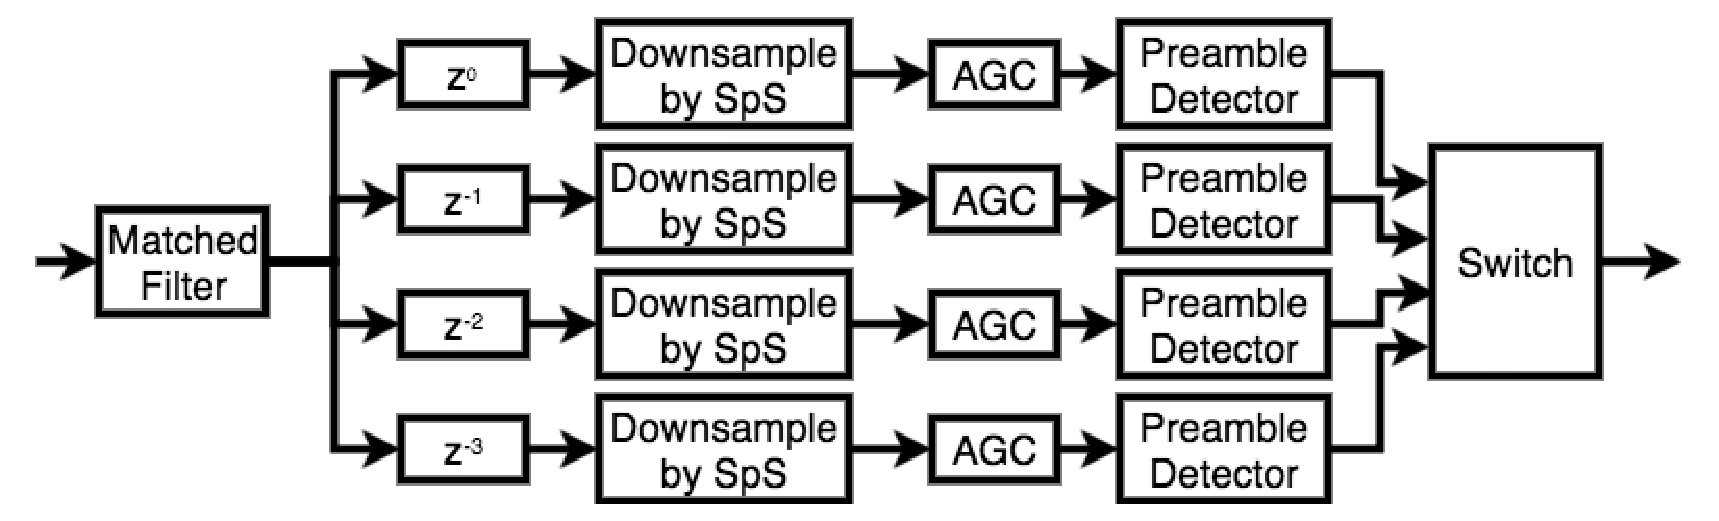
\includegraphics[width=0.95\textwidth]{figures/pncreceiver.eps}
    \caption{Receiver chain.} \label{fig:pncreceiver}
\end{figure}


\subsection{MA receiver, CFO estimation}
To help the receiver estimate CFOs and detect MA transmissions, each frame begins with a Sync preamble and a start of frame delimiter (SFD) part. The sync preamble is a series of zeros and ones, and the SFD is used to verify the detection of a packet.  
%The sync parts are shown in Fig.~\ref{syncs}. 
In our work, the Sync preambles for node A and B are ``1010... 10" and ``0101...01", respectively, which is similar to the packet structure used in the IEEE 802.11 FH PHY.

%\begin{figure} [th]
%    \centering
%    \includegraphics[width=0.3\textwidth]{figure/packet}
%    \caption{Multiple access phase packet structure}\label{ma_packet}
%\end{figure}

Before using the signal to detect a preamble, the signal is passed from an Automatic Gain Control (AGC) unit, in order to normalize the channel gains, $h_1$ and $h_2$.  In a window with a large enough number of symbols, there exists at least one instant that symbols from both sources has an equal or very close phase and have been added constructively. So the AGC adjusts the maximum absolute value of symbols to two. For BPSK,  +1 and -1 represents 1 and 0, respectively. If we index all symbols of the sync part starting from 0, the $k_{th}$ received symbols of Sync preamble can be written as
\begin{equation} \label{maineq}
    s_k=(-1)^{k+1}e^{p_{1,k}} - (-1)^{k}e^{p_{2,k}}.
\end{equation}
For  consistency, we replace all odd indexed symbols of Sync with their additive inverse so the $k_{th}$ symbol can be represented as
%c: mohammad: I cannot understand the above sentence "with their additive inverse..."
\begin{equation}
    s_k^\prime=e^{p_{1,k}} - e^{p_{2,k}}.
\end{equation}
The two phases of $p_{1,k}$ and $p_{2,k}$ can be found by solving the equations below
\begin{equation}
\begin{cases}
    Re(s_k^\prime)=\cos(p_{1,k}) - \cos(p_{2,k}), \\
    Im(s_k^\prime)=\sin(p_{1,k}) - \sin(p_{2,k}).
\end{cases} 
\end{equation}
Since there may be multiple possible answers for these equations,  $p_{1,k}$ and $p_{2,k}$ are chosen in a way that they are closest to $p_{1,k-1}$ and $p_{2,k-1}$ and increasing or decreasing linearly. 

%%%%%%%%%%%%%%%%%%%%%%%%%%%%%%%%%%%%%%%%%%%%%%%%%%%%%%%%%%%%%%%%%%%%%%%%%%%
\iffalse
\begin{equation}
\begin{cases}
    Re(r_i)=-2\sin \left( \frac{p_{1,i}+p_{2,i}}{2}\right)  \sin \left( \frac{p_{1,i}-p_{2,i}}{2}\right), \\
    Im(r_i)=2\sin \left( \frac{p_{1,i}-p_{2,i}}{2}\right)   \cos \left( \frac{p_{1,i}+p_{2,i}}{2}\right).
\end{cases} 
\end{equation}
Then representing $\sin \left( \frac{p_{1,i}+p_{2,i}}{2}\right)$ with $x_{1,i}$ and $\sin \left( \frac{p_{1,i}-p_{2,i}}{2}\right)$ with $x_{2,i}$ we can simplify equations as:

\begin{equation}
    x_{1,i}= \pm \sqrt{\frac{Re^2(r_i)}{Re^2(r_i) + Im^2(r_i)}},
\end{equation}

\begin{equation}
    x_{2,i}= - \frac{Re(r_i)}{2x_{1,i}}.
\end{equation}

the phases can then be found as:
\begin{equation}
    \begin{cases}
        p_{1,i}=k_{1,i} + k_{2,i},\\
        p_{2,i}=k_{1,i} - k_{2,i},\\
    \end{cases}
\end{equation}
where
\begin{equation}
    \begin{cases}
        k_{1,i}= \sin^{-1}(x_{1,i}) \quad or \quad \pi - \sin^{-1}(x_{1,i}), \\
        k_{2,i}= \sin^{-1}(x_{2,i}) \quad or \quad \pi - \sin^{-1}(x_{2,i}),
    \end{cases}
\end{equation}

which leaves four possibilities for answers, each can be tried in (\ref{maineq}) to find the one that matches. 

\fi
%%%%%%%%%%%%%%%%%%%%%%%%%%%%%%%%%%%%%%%%%%%%%%%%%%%%%%%%%%%%%%%%%%%%%%%%%%%

The frequency and phase offsets are then found by a solving a linear regression according to the following equations,
\begin{equation}
    \begin{cases}
        p_{1,k}=(SpS) \omega_1 k + \phi_1, \\
        p_{2,k}=(SpS) \omega_2 k + \phi_2.
    \end{cases}
\end{equation}
\iffalse
where $p_{1,i}^{\prime}$ and $p_{2,i}^{\prime}$ are unwrapped versions of  $p_{1,i}$ and $p_{2,i}$, respectively.
\fi
%
%\begin{figure} [th]
%    \centering
%    \includegraphics[width=0.3\textwidth]{figure/syncs}
%    \caption{Sync preambles. (a) Sync preamble sent by node A . (b) Sync preamble sent by node B}\label{syncs}
%\end{figure}
%
%
%\begin{figure} [th]
%    \centering
%    \includegraphics[width=0.3\textwidth]{figure/sfds}
%    \caption{SFDs. (a) SFD preamble sent by node A. (b) SFD preamble sent by node B. (c) SFD preamble expected in the relay} \label{fig:sfd}
%\end{figure}

\subsection{MA receiver, preamble detection}
A window with the length of the Sync preamble is always sliding on the received samples. Then each time the above CFO estimation algorithm is applied and the $\phi_i$ and $\omega_i$ ($i=1,2$) are used to decode the next $L_{SFD}$ symbols of the packet where $L_{SFD}$  is the length of the SFD part. If the decoded SFD matches the expected SFD, which is XOR of SFD of node A and node B, %Fig. \ref{fig:sfd} (c),
 then the packet is detected and the rest of the symbols are decoded using the same parameters. In our design, SFDs by nodes A  and B are ``1010 0110 1101 0110" and ``1010 1010 0110 1011", respectively, so the SFD expected in the relay is ``0000 1100 1011 1101". 
 
Because of the presence of CFO and phase offset, the constellation is changing from one symbol to another. The right constellation for each received symbol is calculated using the $\phi_i$, and $\omega_i$ and then used for decoding and mapping, According to the mapping function. % as shown in Fig.~\ref{fig:pnc}.
\iffalse you might need to add stuff about the mapping function.\fi



\section{Performance Evaluations}
This section, presents the simulation and experimental results for the PNC transmission. Since the real gain of PNC can been seen in multi-hop transmissions, the same implementation is used for measuring performance parameters in a Multi-hop Physical Layer Network Coding (MPNC). The main MPNC network design used for multi-hop experiments is adopted from \cite{zhang2017cross}. Then using asynchronous experiments the same two hop performance parameters are measured for multi-hop PNC too. 

\subsection{Testbed Experiments}

\subsubsection{Experiment setting}
USRP N210 sets with XCVR2450 daughterboards are used to run the PNC experiments. The software used to develop PNC is GNURadio. The transmission gain of transmitting USRPs is set to $18$~dB and the receiver gain of receiving USRPs is set  to $5$~dB. %The distance between devices is 35Cm and 
The carrier frequency is chosen as $2.45$~GHz. The length of the Sync preamble is $64$ symbols and the $SpS$ used in the experiments is four. 
%When the number of hops is larger than two, the experiment is ran in an asynchronous manner in order to have the right SINR.


\subsubsection{BER, two-hop}
To begin with, we first built a two-hop testbed where two sources A and B exchange the information through a relay, as shown in Figure~\ref{fig:twohoptestbed}. 

Fig.~\ref{fig:e2e_ber} (a) and (b) shows the BER in the MA communications and the end-to-end BER for the two-hop case, respectively. As anticipated, the BER performance deteriorates when the payload length increases, due to the non-stationary wireless channel and the CFOs. Thus, to maintain a low BER,  preambles could be repeated periodically.
%Note that for many machine-type communications with the small-packet feature, packet payload size is quite small, so they fit well with the PNC solutions. 
A somewhat surprising result in Fig.~\ref{fig:e2e_ber} (a) is that there is a small drop of BER around 150-bit block length. This is because, due to CFO, the phase difference of the two transmissions superimposed at the relay changes periodically. \iffalse From  Sec.~\ref{sec:e2eberana}, \fi BER with different phase shift is slightly different. After 100-bit was sent, the phase shift returns to the area corresponding to low BER.  %After an entire cycle, it comes close to the signal again.

\begin{figure} [th]
    \centering
    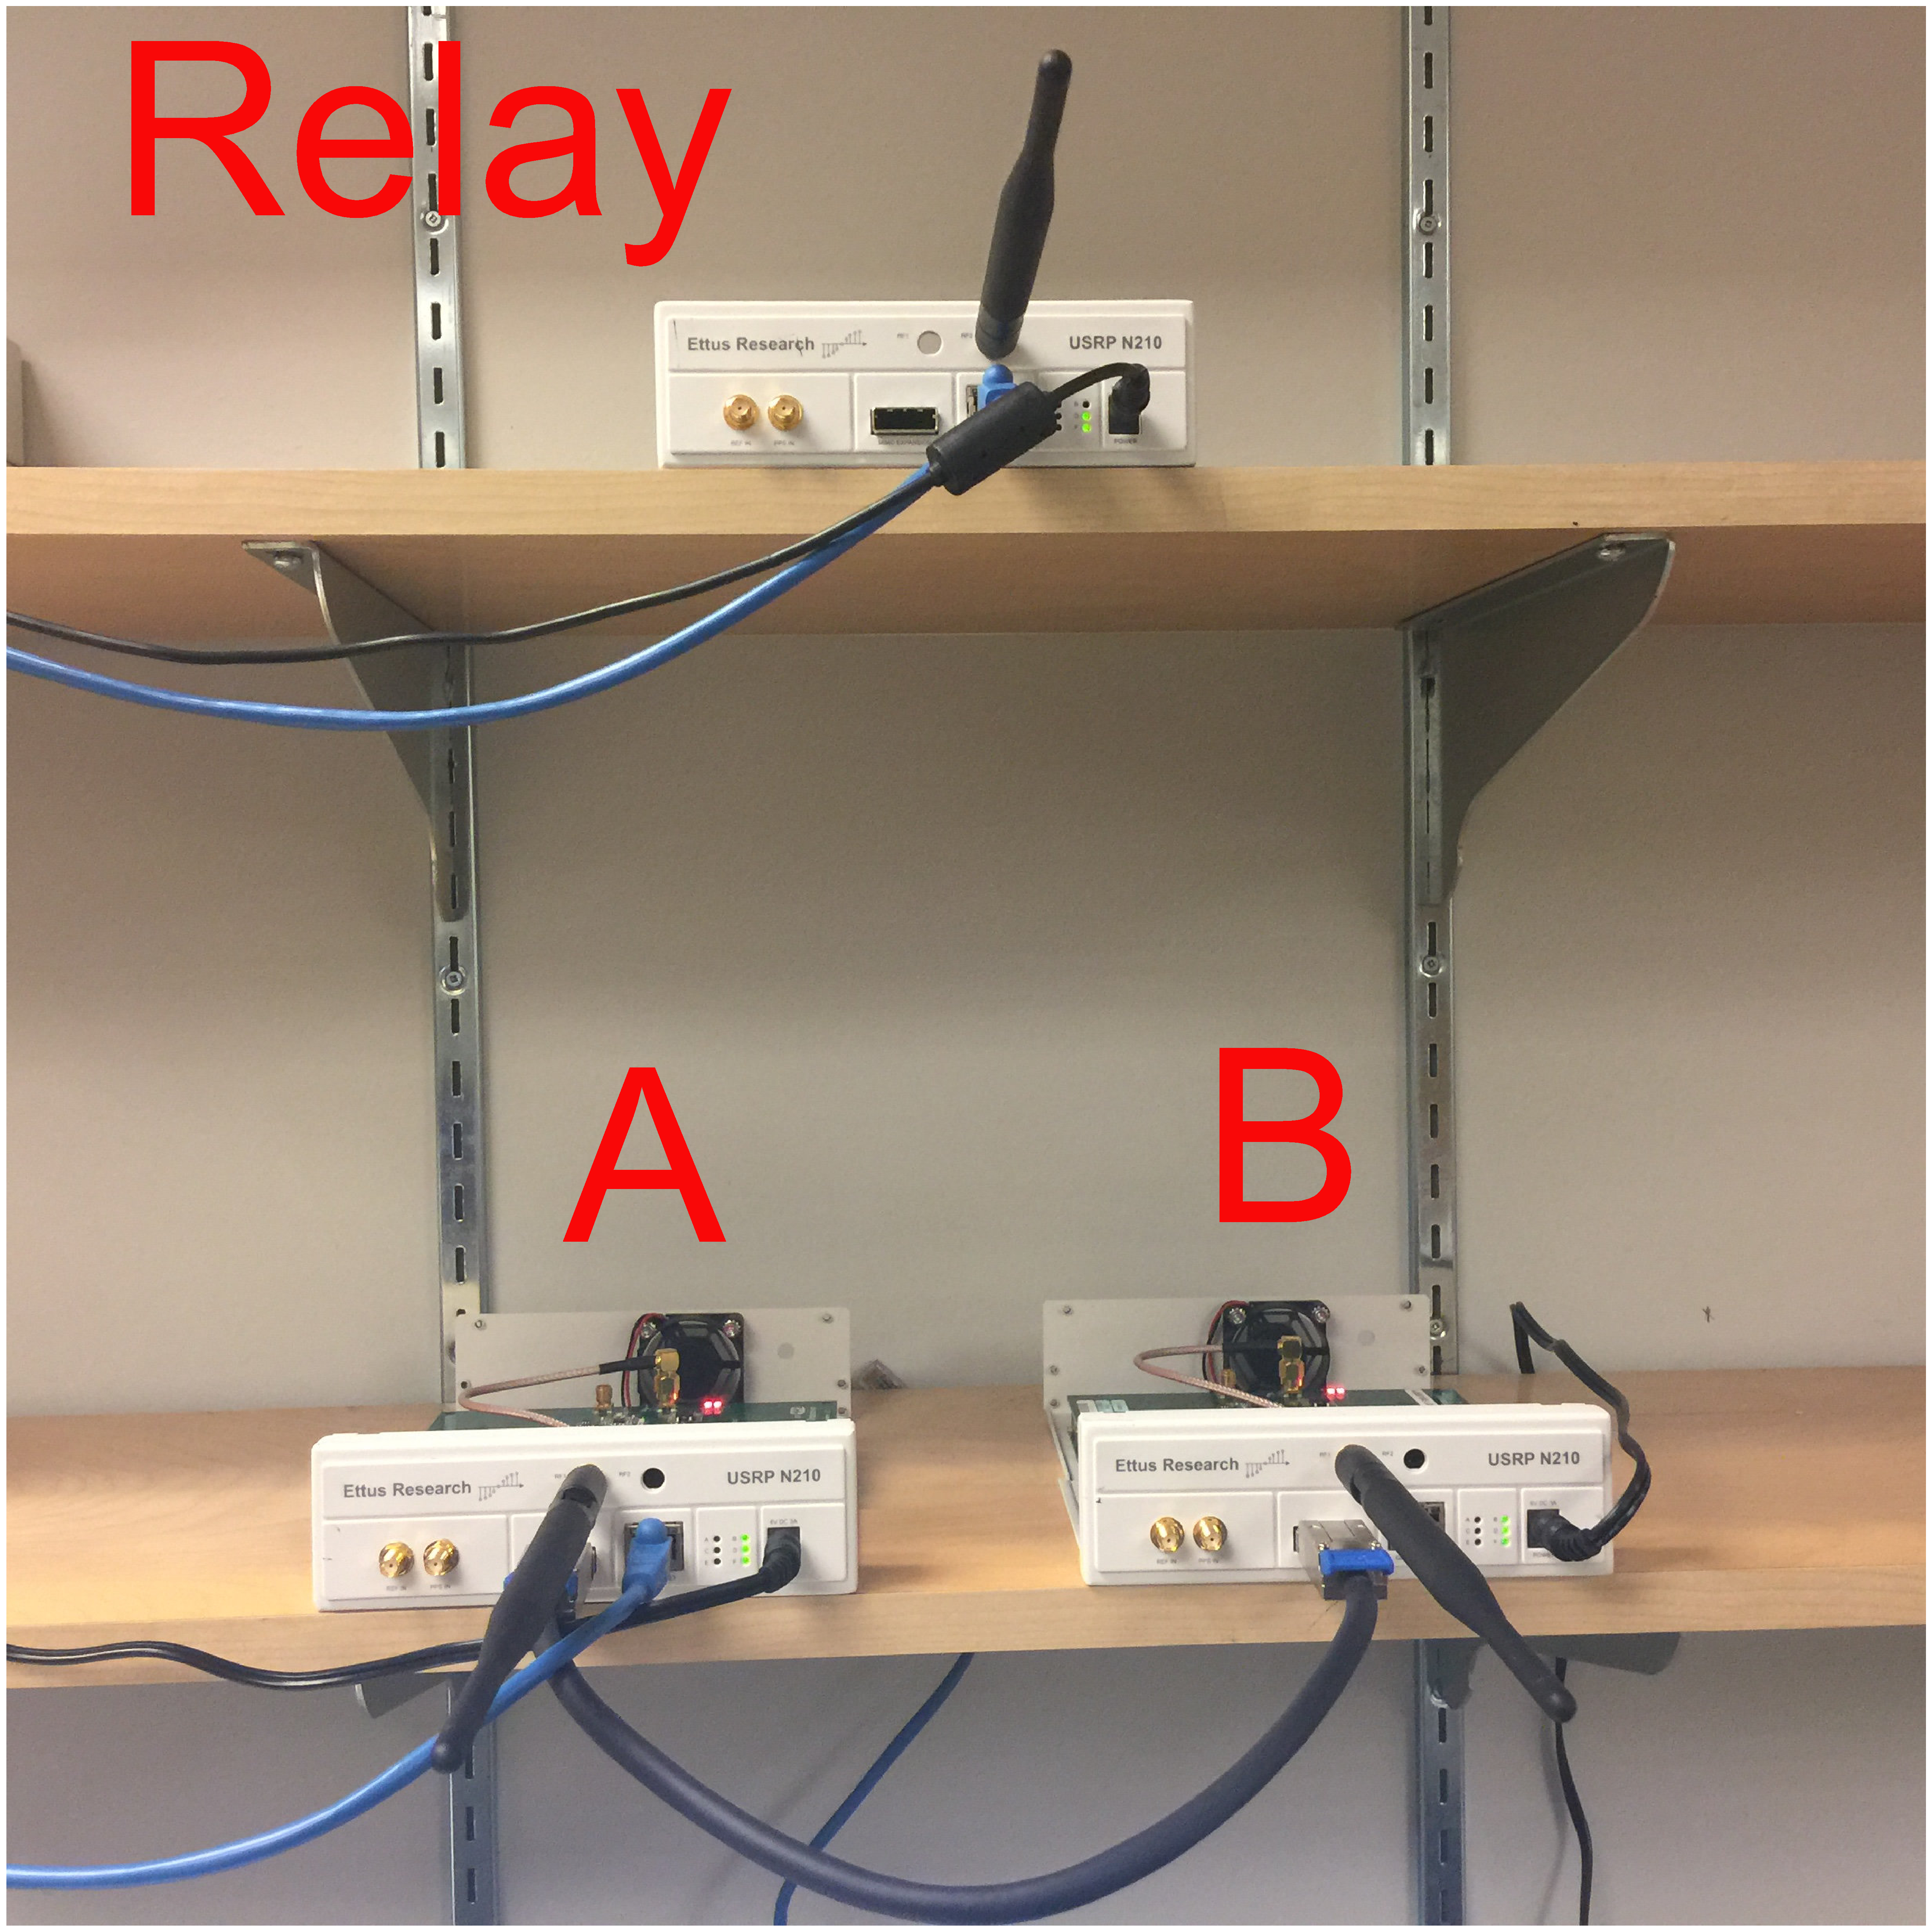
\includegraphics[width=0.95\textwidth]{figures/testbed}
    \caption{Testbed, two-hop scenario.}\label{fig:twohoptestbed}
\end{figure}

%c: mohammad: add the results with 25 bits in. what is the unit of x-axis? bits or bytes? add the unit to the figure.
%                         enlarge the font size 
%                         

%\begin{figure} [th]
%    \centering
%    \includegraphics[width=0.35\textwidth]{figure/cdf}
%    \caption{End-to-end BER, MPNC vs. ANC \cite{katti2007embracing} }
%    \label{fig:cdf}
%\end{figure}

The end-to-end BER results in Fig.~\ref{fig:e2e_ber} (b) include both the MA transmissions and the broadcast transmissions from the relay to the sources. We further compared the end-to-end BER performance of PNC with that of ANC reported in~\cite{katti2007embracing}. The relay in ANC uses an amplify-and-forward approach, instead of the mapping function. From Fig.~\ref{fig:e2e_ber} (c),  MPNC slightly outperforms ANC, from the USRP testbed experiments. In general, the performance of amplify-and-forward degrades in the low SINR region. 

\begin{figure*} [th]
\centering
\begin{tabular}{ccc}
    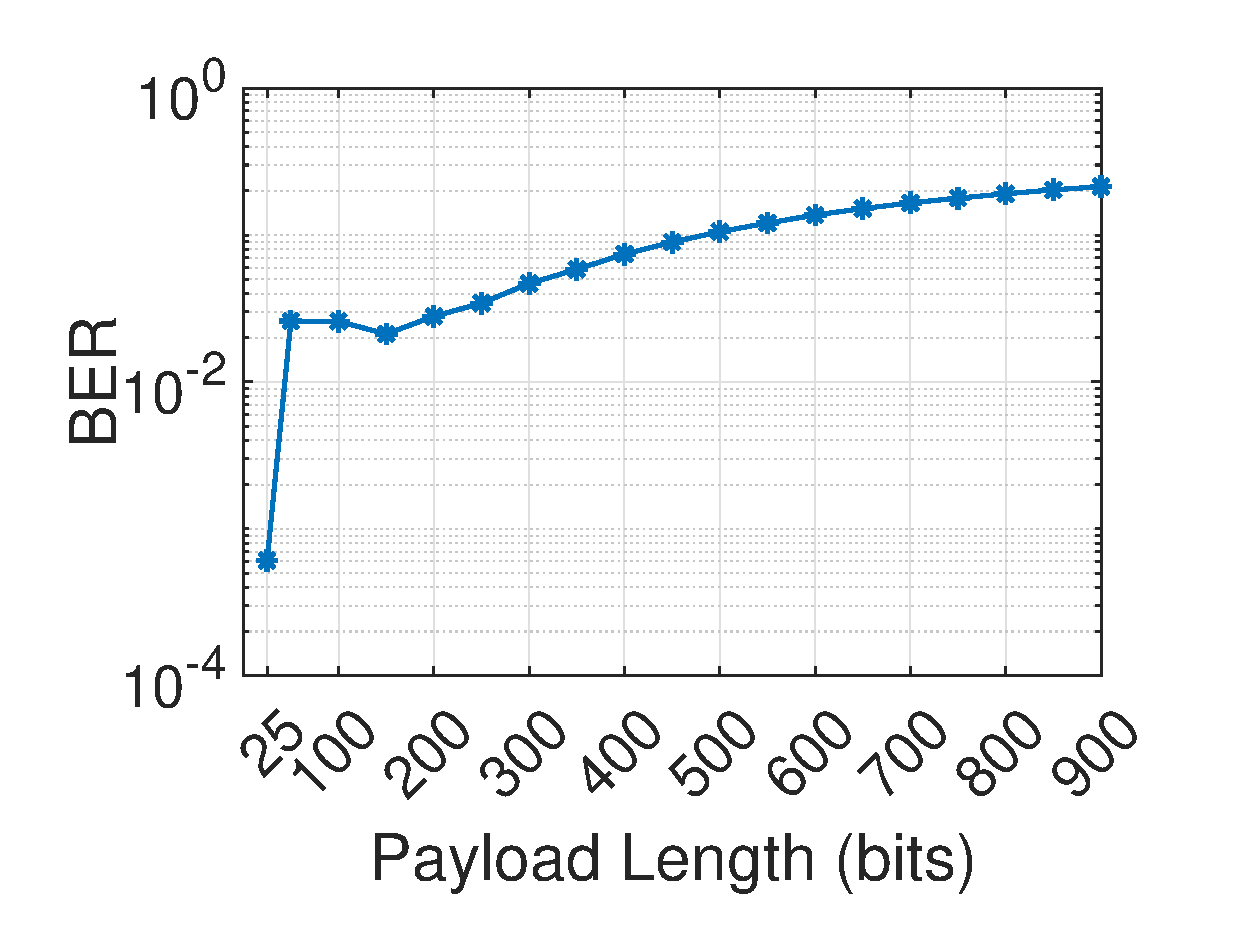
\includegraphics[width=0.33\textwidth]{figures/BER_Payload_MA.eps} &
    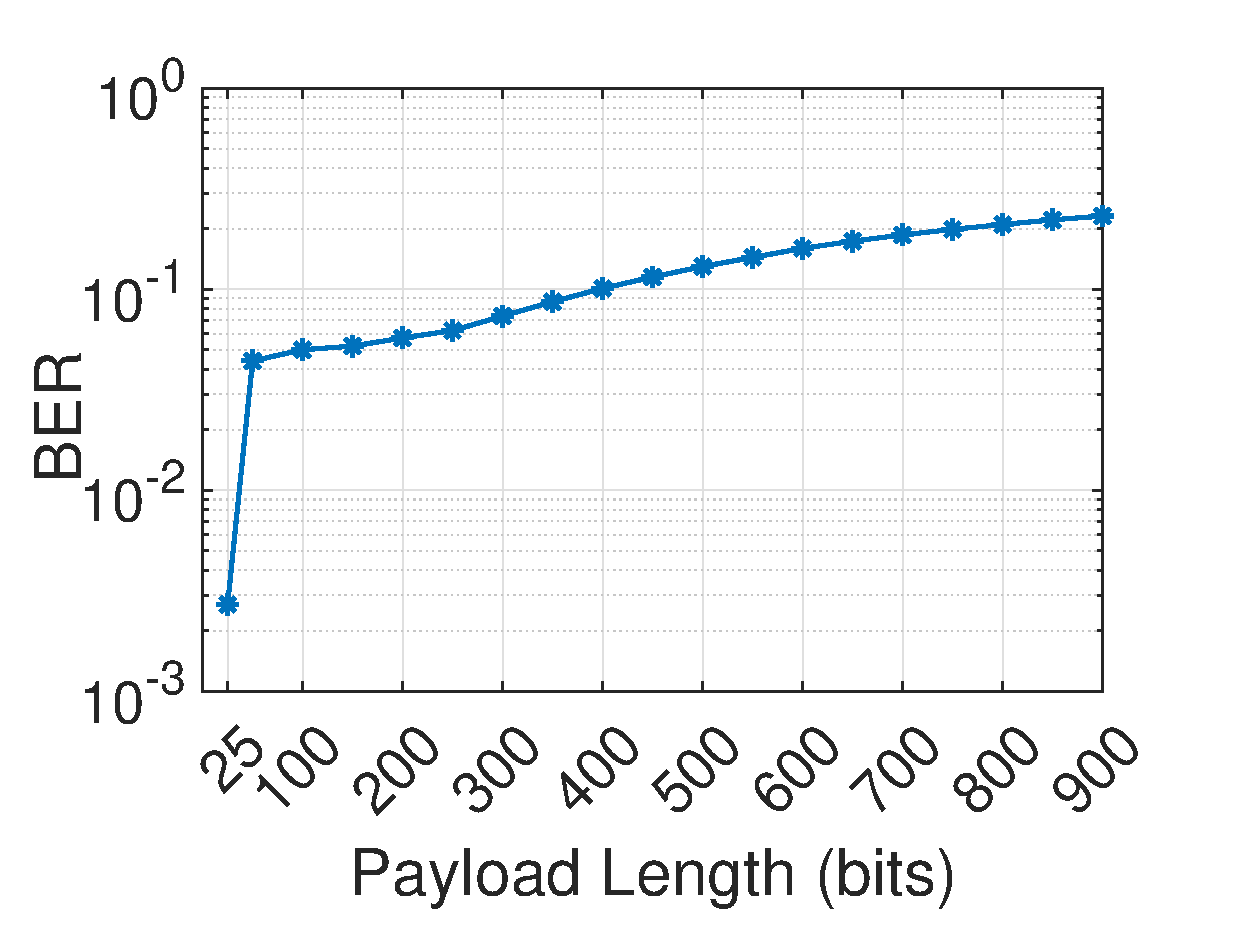
\includegraphics[width=0.33\textwidth]{figures/BER_Payload_e2e.eps}&
     \includegraphics[width=0.33\textwidth]{figures/cdf}\\
      (a) MA  transmission BER &    (b) End-to-end BER & (c) MPNC vs. ANC
      \end{tabular}
       \caption{BER performance, two-hop.}
    \label{fig:e2e_ber}
\end{figure*}

\begin{figure} [th] 
\centering
\begin{tabular}{cc}
   \hspace*{-12pt} 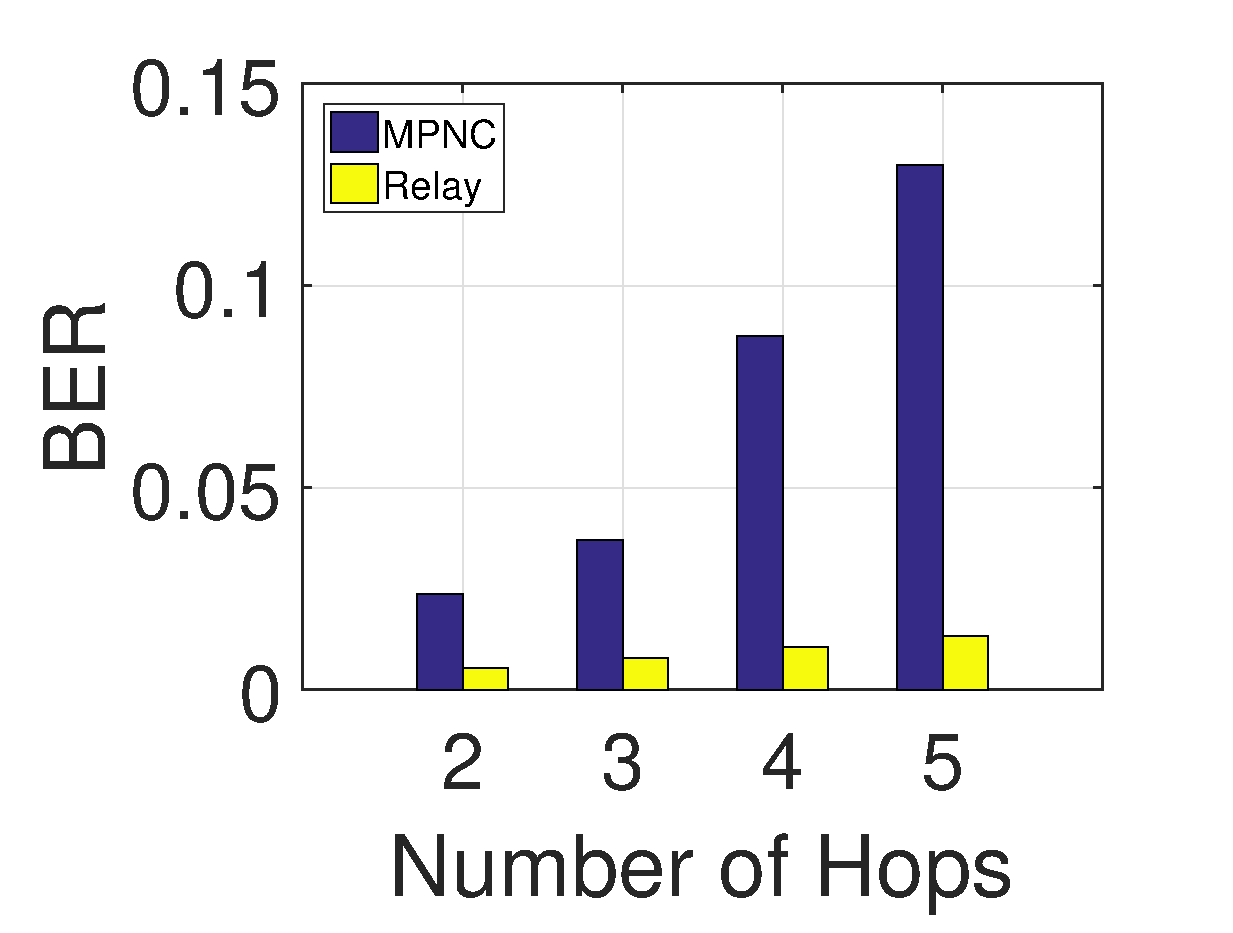
\includegraphics[width=0.47\textwidth]{figures/ber_bar_160}&
   \hspace*{-12pt}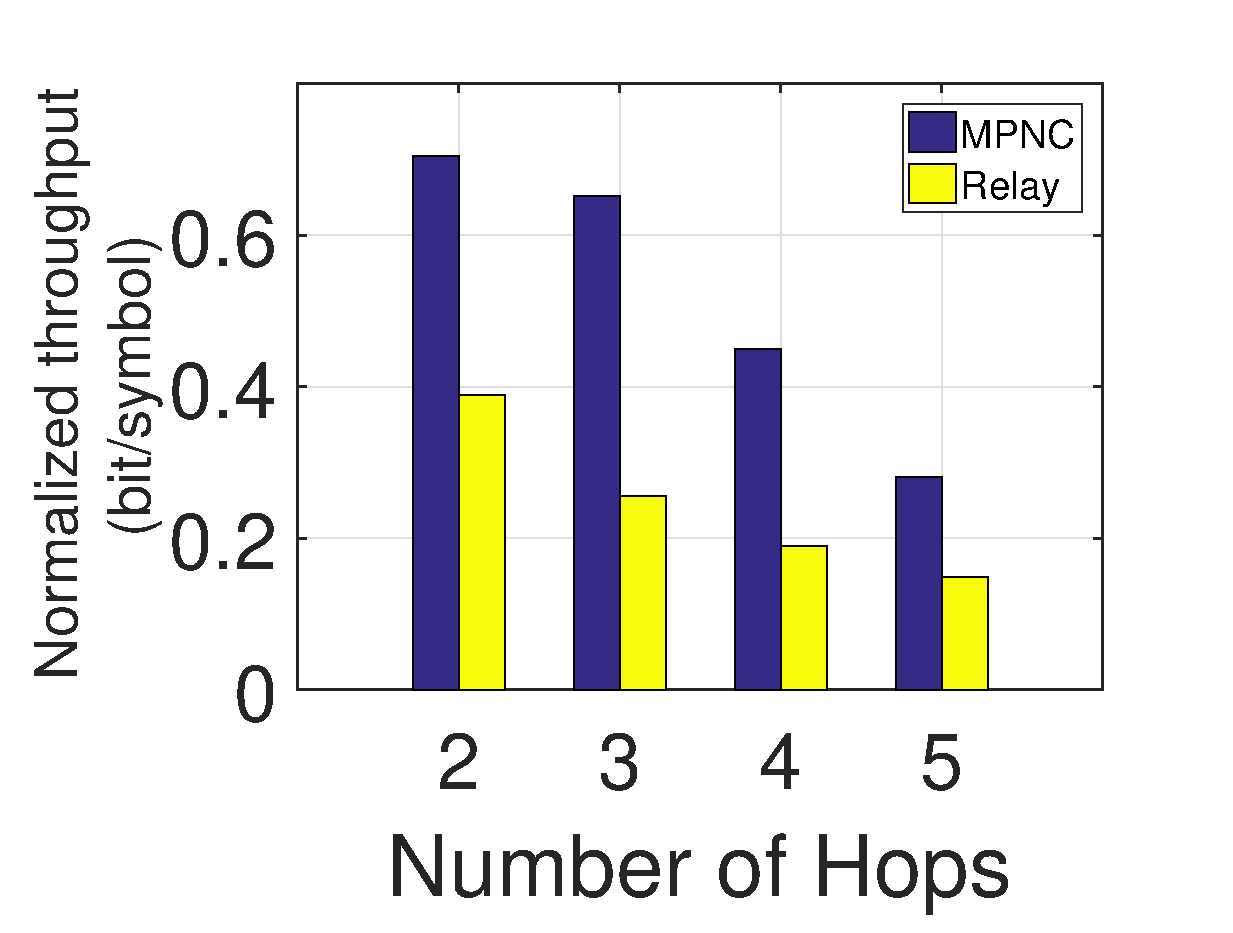
\includegraphics[width=0.47\textwidth]{figures/th_bar_160}\\
      \hspace*{-12pt} (a) End-to-end BER &
 \hspace*{-12pt} (b) Normalized throughput
      \end{tabular}
       \caption{Multi-hop performance. Multi-hop End-to-End BER are calculated using formulations outlined in table 5.1 of \cite{zhang2017cross}.} %(payload = 160 bits)}
    \label{fig:experiment_ber}
\end{figure}

\subsubsection{Multi-hop performance}
Next, we extended the two-hop scenario to multi-hop scenario, where the number of hops varied from two to five. The transmission and reception of the relays for multiple hops behave similarly as that in the two-hop case, except that the mutual interference  and the error propagation problem will lead to a higher BER.

Figs.~\ref{fig:experiment_ber} (a) and (b) compare the end-to-end BER and normalized throughput, respectively of MPNC and that with hop-by-hop relay. 
The normalized throughput is the number of bits successfully received by the destination per symbol duration. 
From the figures, although the end-to-end BER of MPNC is much higher than that of hop-by-hop relaying, due to both the worse BER performance in MA transmissions and the error propagation problem (i.e., a single MA transmission error may affect multiple end-to-end bit errors in a multi-relay path),  the end-to-end throughput of MPNC is much higher
than that of hop-by-hop relay. Using the inexpensive USRP testbed, it is encouraging to notice that the performance gain of MPNC ranges from $75\%$ to $80\%$ for the two- and five-hop cases, and around $150\%$ for the three- and four-hop cases. 


%comparing the two graphs reveals that although end to end BER of MPNC can go much higher than hop by hop relaying, due to its nature of exchanging two packets in two slots with any number of hops, it can always maintain a throughput higher than hop by hop relaying. The throughput of MPNC is also compared to other mechanisms of multi-hop relaying in \ref{sub:throughput} using simulation results.

  



%%%%%%%%%%%%%%%%%%%%%%%%%%%%%%%%%%%%%%%%%%%%%%%%%%%%%%%%%%%%%%%%%%


\subsection{Simulation Results}

To evaluate and compare the performance of the proposed MPNC in controllable and repeatable environment with a wide range of settings, we used Matlab and GNURadio to conduct extensive simulations and the results are presented in this section. 

%In this section, the performance of the proposed multi-hop PNC scheme is evaluated using excessive simulations. Also the effect of multiple parameters that are not controllable in practice is studied. Matlab and GNURadio are softwares used to run simulations. 

\iffalse

\subsubsection{Different number of hops} % (fold)
\label{sub:awgn}
In this subsection, we study the end-to-end performance considering different number of hops, aiming to identify the optimal number of hops. 
For fair comparison, here, we let the total transmission power in any two continuous slots be $2E_b$, and all the nodes equally share the total transmission power. In other words, if the number of hops increases, the transmission power per node decreases accordingly. The nodes are located in a linear topology with equal distance for each hop.  The average received SNR of all links are proportional to $d^{-\alpha}$, where $d$ is the hop distance. %We studied the performance of MPNC under AWGN channel with different path-loss parameters.

\begin{figure*} [th]
    \centering
    \subfloat[][$\alpha = 4$.]{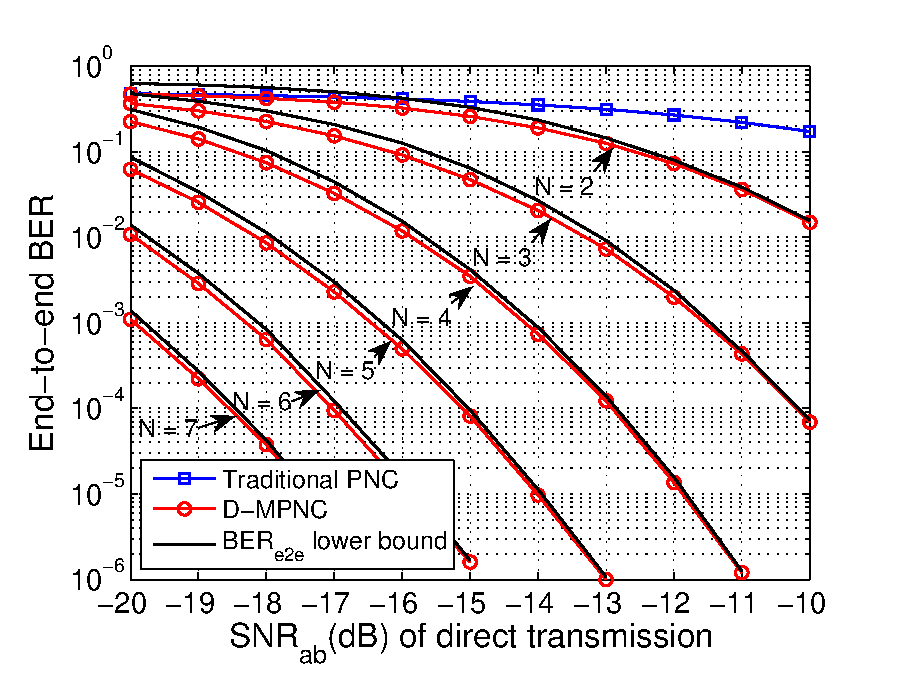
\includegraphics[width=.34\textwidth]{figures/dmpnc_alpha_4_awgn.eps}}
    \subfloat[][$\alpha = 3$.]      {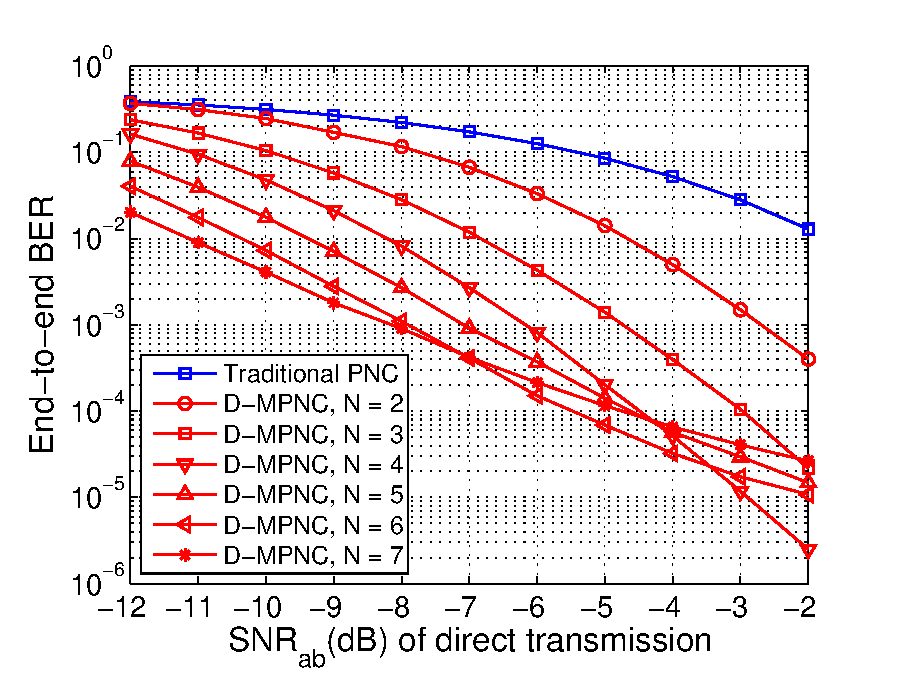
\includegraphics[width=.34\textwidth]{figures/dmpnc_alpha_3_awgn.eps}}
    \subfloat[][$\alpha = 2$.]      {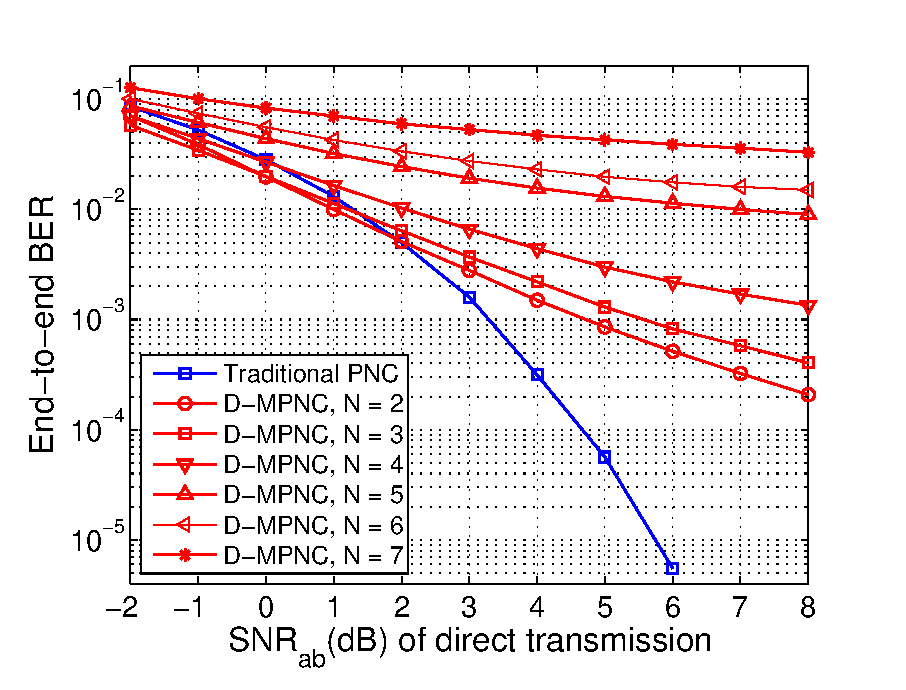
\includegraphics[width=.34\textwidth]{figures/dmpnc_alpha_2_awgn.eps}}
    \caption{End-to-end BER performance of MPNC under AWGN channel.}\label{ber-D-MPNC}
\end{figure*}
%c: haoyuan: change D-MPNC to MPNC in the figures, and change "lower bound" to "bound". 

Since the end-to-end data exchange rate of PNC and MPNC remains the same no matter how many relays are used, we only need to compare the end-to-end BER performance. 
The end-to-end BER results considering different number of relays and different path loss exponents are shown in Fig. \ref{ber-D-MPNC}. The X axis is the end-to-end $\text{SNR}_{ab}$(dB) by direct transmission (without any relay). The \textit{Traditional PNC} curves are for the case with one relay only so the traditional PNC solution can be directly applied. 
With $N$ relay(s), the transmission power per node is  less while the path loss also reduces. The mutual interference also increases when the number of relays increase. Therefore, there is a tradeoff, and the optimal number of hops largely depends on $\alpha$, typically  ranging  from $2$ to $6$~\cite{goldsmith2005wireless}. 
%Given the end-to-end $\text{SNR}_{ab}$(dB) in (\ref{end-to-end-snr}) and the distance $d$(m) between the sources, the larger $\alpha$ is, the SINR(dB) of each hop in (\ref{sinr}) is larger by shortening the transmission path. Another impact is that a larger $\alpha$ reduces the impacts of the inference from other transmitting nodes to the receiver due to a larger path loss. The impacts of the path-loss parameter $\alpha$ is also studied in this section.

In Fig. \ref{ber-D-MPNC}(a), the black curves are the  end-to-end BER bound of MPNC obtained in Table~\ref{L_D_MPNC} and the red circled curves are the simulation results. When the BER is low, the bound and the simulation results converge. This is because,  when the BER is low, the probability that  more than one multi-access and single-hop errors occur in a slot becomes negligible. Comparing Figs. \ref{ber-D-MPNC}(a), (b) and (c),  $\alpha$ has a great impact on the end-to-end BER performance. In Fig. \ref{ber-D-MPNC}(a), when $\alpha=4$, MPNC outperforms the traditional PNC with single relay significantly due to the a relatively larger SINR between the neighbor nodes as the interference and signal strength both decay fast with distance. The tendency also shows that with the lower end-to-end SNR (or larger distance between the sources), we can add more relays to ensure that the BER is below a threshold.
In Fig. \ref{ber-D-MPNC}(c), when $\alpha=2$, the two-hop PNC achieves the best performance when the end-to-end SNR is above $2$~dB; and below that, all solutions perform poorly.  
In Fig. \ref{ber-D-MPNC}(b), when $\alpha=3$, the optimal number of relays depends on the end-to-end SNR (or distance). 
%In Figs. \ref{ber-D-MPNC}(b) and (c), with the increase of end-to-end $\text{SNR}_{ab}$(dB), the end-to-end BER performance converges with a larger relay number $N$. Because the interference from other transmitting nodes in multi-hop PNC also increase with the increase of $\text{SNR}_{ab}$(dB), and the SINR of two neighbor node approach to the upper bound. Further increase $\text{SNR}_{ab}$(dB) will not help to improve the end-to-end BER, as the SNR of each hop is upper bounded by $10\alpha\log_{10}{3}$(dB) as explained in Sec. \ref{sec-inter}.
The results suggest that when $\alpha$ is large (e.g., $\ge3$), we can apply MPNC to solve long-distance wireless transmissions using a large number of relay. 

\fi




\subsubsection{Goodput performance comparison} % (fold)
\label{sub:throughput}


In this section, the goodput of MPNC is studied and also compared with the other state-of-the-art solutions. As we compare the performance of different solutions with the same number of hops, different from the last subsection, here, the transmission power of each node and the hop distance remains constant. %For MPNC, Hop by hop, and Full Duplex solutions, we
The goodput measures the number of error-free packets received per slot.
% is defined as 
%\begin{equation}
%   Th=1-(1-BER)^{Payload Length}\frac{2}{S_k},
%\end{equation}
% where $S_k$ is the number of slots required to exchange $k$ packets. 
For the full-duplex relay solution, in the simulation, we made a strong assumption that the self-interference can be fully cancelled. Thus, the performance shown in our simulation can be viewed as the upper bound of it. 
As the existing PNC method for multi-relay path suffers from the infinite error propagation problem, to make it usable, after detecting each error, the destination must  notify all other nodes and the pipeline should be   flushed and restarted. The goodput for the PNC method is thus affected by the restarts.
Note that with the infinite error propagation problem, an error detection coding have to be used for PNC, but the error correction coding cannot be applied, which is a severe disadvantage for it. 
 
% calculated by
% \begin{equation}
%   Th_{PNC}\sum_{k=1}^{\infty} \frac{2k}{S_k} P_{s,k}^{PNC} P_{e}^{PNC},
% \end{equation}
% where $P_{s,k}^{PNC}$ the probability of successfully exchanging $k$ packets using PNC method and $P_{e}^{PNC}$ is the probability of an error happening while exchanging two packets.


The goodputs  are shown in Fig.~\ref{fig:throughputPNC}. Comparing with the other state-of-the-art algorithms, MPNC has always a higher goodput and can maintain its performance as the number of hops increases. The goodput gains of MPNC over hop-by-hop relay, full-duplex, and PNC is about 3x times, $33\%$, and $68\%$ when the number of hops is as high as eight. Also, from the figure, the goodput of MPNC remains close to 0.9 packet/slot when the number of hops varied from two to eight, showing that it is quite scalable to long paths. 

% subsection throughput (end)


\subsubsection{Effect of CFO on BER} % (fold)
\label{sub:effect_cfo_on_ber}
Fig.~\ref{fig:cfo} (a) shows the impacts of CFOs on the BER performance.
 High CFO is set according to the practical number measured from the USRP devices in our testbed, and the low CFO is 0.1 of that. As it can be seen in the figure, CFO compensation is crucial to the performance of MPNC. The figure shows that when CFO is not compensated, the performance is poor (larger than $10\%$ bits in error) no matter whether the CFO is high or low. On the other hand, using the proposed CFO compensation algorithm can improve the BER performance significantly.

 %Average CFO compensation is when the average value of CFO is used for both $f_1$ and $f_2$.
 % The key result is that although estimating CFO of both nodes with their average and attempting to remove its effect by a multiplication can have a good performance with low CFO values, the algorithm proposed in this paper can maintain a better and lower BER as payload %length increases. The reason for that is because the average CFO method does not remove the effect of CFO completely and a small rotating phase remains in both signals which causes a higher number of errors for large payload lengths.

\begin{figure} [th]
    \centering
    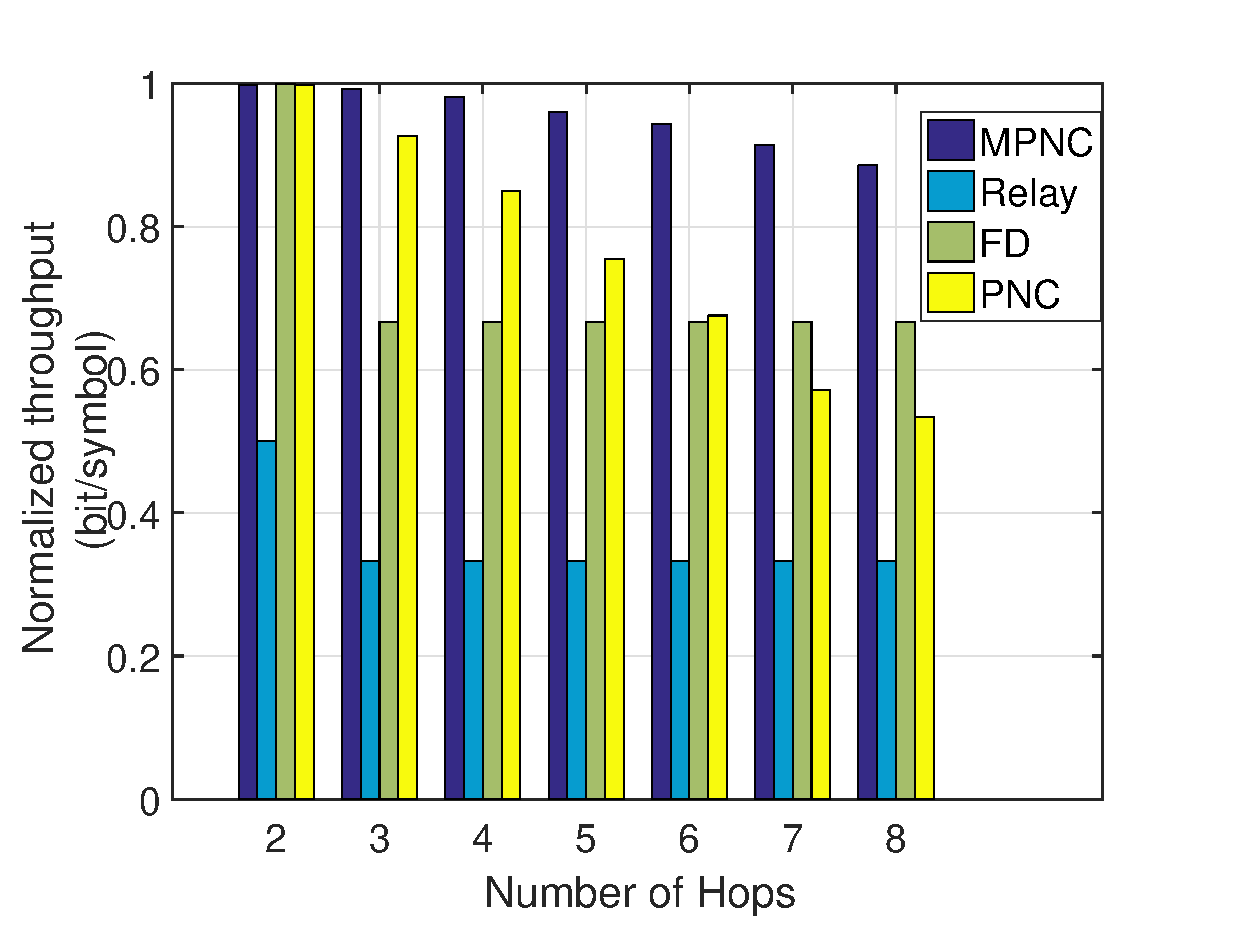
\includegraphics[width=0.95\textwidth]{figures/sim_th_alpha4_snrh2h9BL256}
    \caption{Goodput, per-hop SNR $=9$, $\alpha=4$, Payload=$256$ bits.}
    \label{fig:throughputPNC}
\end{figure}

% subsection effect_cfo_on_ber (end)


\subsubsection{Effect of Channel Estimation Error on BER} % (fold)
\label{sub:effect_of_channel_estimation}
We studied the effect of channel estimation error %which can also be interpreted as having relays on not perfect location, 
on end-to-end BER performance. In Fig.~\ref{fig:cfo} (b), $\delta$ represents the ratio of estimated channel gain and the real channel gain. From the figure, 
overall, the BER increases when the channel estimation error increases,  while  the algorithm can maintain a reasonable BER even with $10\%$ to $20\%$
estimation errors. 
%\begin{figure} [th]
%    \centering
%    \includegraphics[width=0.25\textwidth]{figure/locations2_new}
%    \caption{Effect of Channel Estimation Error on BER}
%    \label{fig:channel_estimation}
%\end{figure}
%c: instead of using alpha, which has been used as path loss exponent, use $\delta$ here. 
% why the 0.8 curve and 0.9 curve cross at 100 bit? 

% subsection effect_of_channel_estimation (end)

\begin{figure} [th] 
    \centering
  \begin{tabular}{cc}  
    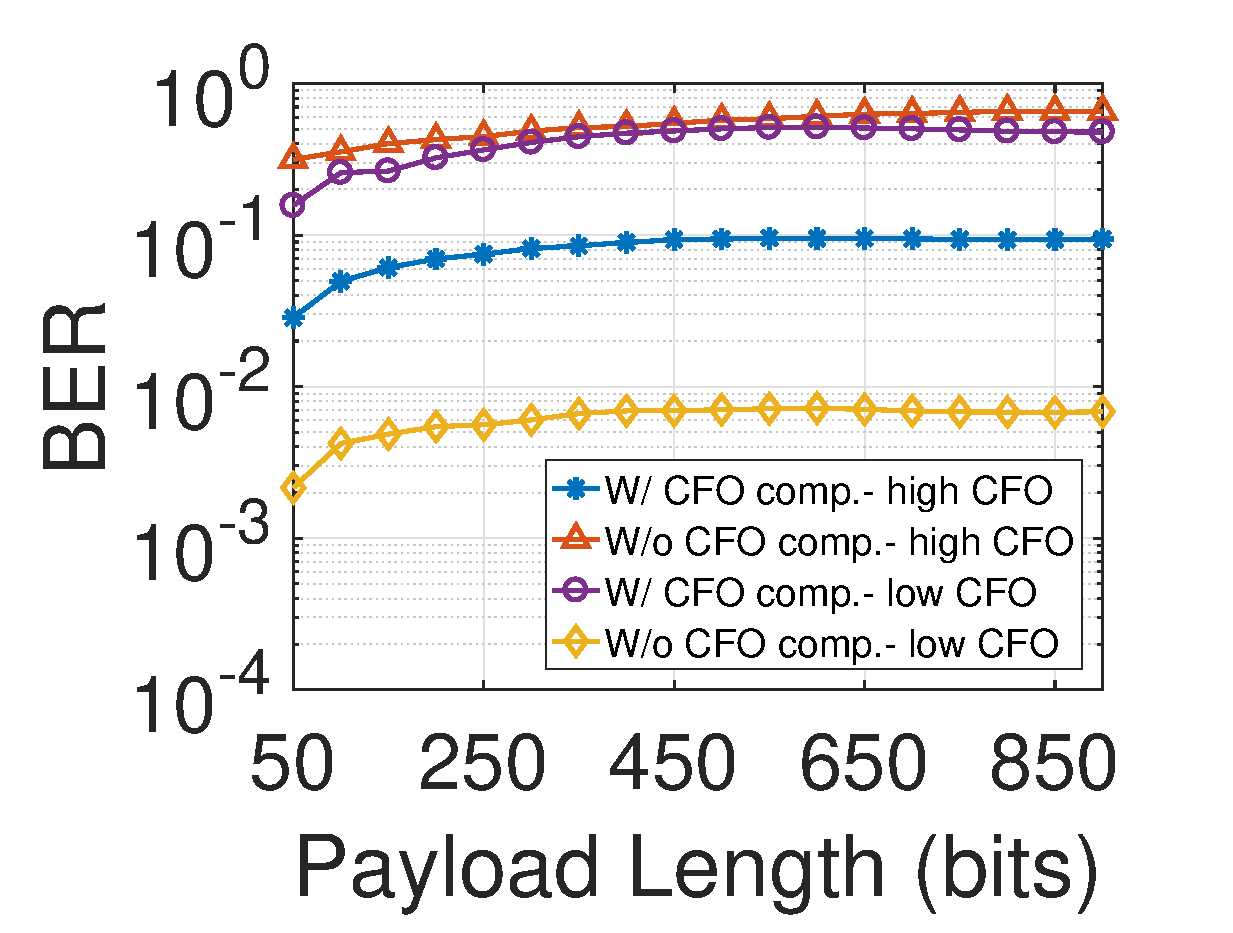
\includegraphics[width=0.47\textwidth]{figures/cfo2} &
     \includegraphics[width=0.47\textwidth]{figures/locations2_new}\\
     (a) CFO compensation & (b) Channel estimation error
     \end{tabular}
    \caption{Effect of CFO and channel estimation error on BER. }
    \label{fig:cfo}
\end{figure}